\documentclass[pdftex,10pt,a4paper,oneside]{article}
\usepackage[English]{babel}
\usepackage{amsmath} %For both in-line and equation mode
\usepackage{listings}
\numberwithin{equation}{section} %Numbering of our equations per section
\usepackage{graphicx} %Inserting images
\usepackage{pgf, tikz}
\usepackage{paralist}
\usepackage{enumerate} 
\usepackage{setspace} %Spacing on the front page for crest and titles
\usepackage[hyphens]{url} %Deals with hyphens in urls to make them clickable
\usepackage{color}
\usepackage{amsthm}
\usepackage{float} 
\usepackage{subcaption}
\definecolor{dkgreen}{rgb}{0,0.6,0}
\definecolor{gray}{rgb}{0.5,0.5,0.5}
\definecolor{mauve}{rgb}{0.58,0,0.82}
\usepackage{algorithm}
\usepackage{algorithmic}

\lstset{frame=tb,
   language=Python,
   aboveskip=3mm,
   belowskip=3mm,
   showstringspaces=false,
   columns=flexible,
   basicstyle={\small\ttfamily},
   numbers=none,
   numberstyle=\tiny\color{gray},
   keywordstyle=\color{blue},
   commentstyle=\color{dkgreen},
   stringstyle=\color{mauve},
   breaklines=true,
   breakatwhitespace=true
   tabsize=3
   }

\begin{document}

% !TEX root =  ../Report.tex

\thispagestyle{empty}

\begin{spacing}{2}
	\begin{center}
		
\includegraphics[scale = 0.25]{Preamble/logo.png}
	\end{center}
	\vspace{5mm}
	\begin{center}
		\textbf{\begin{LARGE}
		CS440: Project 1
		\end{LARGE}}
		\vspace{5mm}
	\end{center}
	\begin{center}
		{\large Fast Trajectory Planning}\\
		\vspace{20mm}
	\end{center}
	\begin{center}
		\textbf{\large Alborz Jelvani}
		\vspace{20mm}
	\end{center}
	\begin{center}
	     {\large Professor: Rui Wang}\\
		\textbf{\large Department of Computer Science}\\
		{\large Rutgers, The State University of New Jersey}\\
		{\large July 2020\\}
	\end{center}
\end{spacing}

\pagenumbering{roman}


\textbf{
For further references on code, please refer to:
\linebreak
\url{https://github.com/Jelvani/Rutgers_CS440_Intro_to_AI}
}
\section{Introduction}
\label{sec:Introduction}

In this project, we will first perform an analysis of the classical $A^* search$  algorithm. To begin, it is important to define our environment and testing conditions. All tests are performed on a 101 X 101 grid where each cell is considered an atomic unit of the map. The map world is defined to be \emph{static} and initially \emph{unknown}, meaning the cells that are walls do not change as the \emph{agent} moves and the location of the walls is initially unknown. The agent can start at any cell for its \emph{initial state} and the agent is to navigate the \emph{partially observable} environment. That is, the agents \emph{actions} include checking any adjacent cells for walls and moving to any adjacent cells.


Now We will briefly explain our implementation details with Python that are required for this problem. Our \emph{state space} consists of all reachable cells from the initial state, and we will therefore need a way to store each state along with the path taken to reach that state. We provide a \texttt{Node} class that looks like the following:
\begin{figure}[h]
\begin{lstlisting}
class Node():
    def __init__(self,parent = None,position = None,g = 0,h = 0):
        self.parent = parent #type Node
        self.position = position #type tuple
        self.g = g
        self.h = h
    def __eq__(self, otherNode): #for '==' comparison of a Node object
        return otherNode.position == self.position
    def __lt__(self, otherNode): #for '<' comparison of a Node object
        if self.f == otherNode.f:
            return self.g >= otherNode.g #tie breaker for same f value
        else:
            return self.f < otherNode.f
    @property
    def f(self):
        return self.g + self.h
\end{lstlisting}
\caption{A Python implementation of the \texttt{Node} class, which is created for each cell in our open list.}
\end{figure}


It is important to note our parent variable, which is type \texttt{Node}. This will allow us to create a linked list that represents the path taken to reach the current node. Furthermore, we will use the \texttt{Numpy} library for creating our binary 101 X 101 matrix that will represent our map with walls. The \texttt{Numpy} library also lets us easily store our generated mazes for future use. It is also important to have a efficient data structure for the priority queue required by $A^* search$. We will discuss $A^*$ in more depth in later sections, but since we need to explore the node with the smallest evaluation function, given by $f(n) = g(n) + h(n)$, we do not want to iterate over all values in the open list containing the nodes. Therefore, we use the \texttt{heapq} library, which implements a binary heap. This is also why we provide the \texttt{lt} definition in our \texttt{Node} class, since it is used by Python has an overloading operator for the \emph{less than} operator so the \texttt{heapq} library can maintain the binary heap data structure. Compared to a normal linear search with a worst case run time of $\mathcal{O}(n)$, a binary heap will give us the lowest evaluation function valued node in $\mathcal{O}(\log n)$ worst case run time.

For visualization purposes we will use the \texttt{matplotlib} library. This allows us to view our \texttt{numpy} arrays on a graph and will also help us save the generated graphs to an image file.



\emph{** Update: For this paper, figures displayed were using }\texttt{matplotlib}. \emph{In the latest version of the repository, the} \texttt{pygame} \emph{library is used.}
\section{Experimental Setup}
\label{sec:Experimental Setup}
All tests are performed on the following machine:
\begin{itemize}
  \item OS: Windows 10 Enterprise version 1903
  \item CPU: Intel Core i7-4790 @ 3.60 GHZ
  \item RAM: 16.0 GB
  \item Python Version: 3.8.2 (32-Bit)
\end{itemize}
All run times shown are in seconds, and timing is calculated with Pythons built-in \texttt{time} module. For run-time testing, any print functions that are used in-between timings are disabled, as well as any plotting functions. For each search in a maze, the start and goal coordinates are kept at a constant $(0,0)$ and $(100,100)$ respectively.
% !TEX root =  ../Report.tex

\section{Part 0: Setup your Environments}
\label{sec:Part 0} 
To begin this project, we provide 2 methods of maze generation. The first method is the simplest, and is implemented in our \texttt{createRandMaze()} function. Calling this will create a 101 X 101 boolean matrix and with a probability of 0.2, each cell is a wall. This generated numpy array is then saved once as a text file and once as a matplot figure image.

Our second method of maze generation is more sophisticated and implemented in our \texttt{createBtrackingMaze()} function. This function will use the \emph{Depth First Search} algorithm to carve a path through a boolean numpy array of all walls. After it hits a dead end, it will then backtrack its way out and create another path. The advantage of this method, is that it creates the perfect maze. Every open cell in the array can be reached by any other open cell.
\begin{figure}[H]
\begin{subfigure}{.5\textwidth}
  \centering
  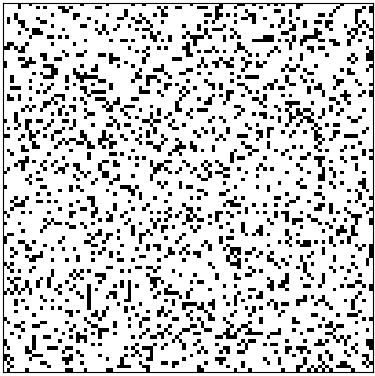
\includegraphics[width=0.8\linewidth]{Report/Part0/random.png}  
  \caption{Random maze}
\end{subfigure}
\begin{subfigure}{.5\textwidth}
  \centering
  
\includegraphics[width=0.8\linewidth]{Report/Part0/backtracked.png}  
  \caption{DFS backtracked maze}
\end{subfigure}
\caption{Sample maze generations}
\end{figure}

Using the above 2 methods, we will generate 25 random mazes and 25 backtracked mazes for our tests. As mentioned previously, we will also save these to file so the same mazes are used for all of our tests.
% !TEX root =  ../Report.tex

\section{Part 1:  Understanding the methods}
\label{sec:Part 1} 
Now that we have discussed how we will be generating our mazes, we will first discuss the concept behind $A^* search$, and other search methods that exist.


$A^* search$ is an \emph{informed search} strategy. This means that the agent has some knowledge about where the goal state is relative to all other states in the state-space. This is opposed to \emph{uninformed search} strategies, which means the agent is blind about any information for a state, other than the provided problem definition. In other words, this means that an informed search strategy would require information, such as the distance from each state to the goal state, to function properly, where an uninformed search strategy would not need this. The advantage of using an informed search strategy is that the algorithm is much more intelligent and can arrive at the goal in less time as opposed to uninformed search strategies.


This extra information informed search strategies require is often used to feed something called an \emph{evaluation function}, $f(n)$. The definition of $f(n)$ depends on the informed search strategy used, but what we are concerned with is $A^* search$, which has the evaluation function of $f(n) = g(n) + h(n)$, where $h(n)$ is know as our \emph{heuristic function} and $g(n)$ is the cost to reach the current state from our initial state.


As mentioned before, informed search relies on extra information about the states and the goal, and this is where our heuristic function comes into play. $h(n)$ is the distance from each state to the goal state, and it must be \emph{admissible} for $A^* search$ to work properly. This means that $h(n)$ must never overestimate the cost of reaching the goal from state $n$. For any 2 points, an admissible heuristic is often the \emph{euclidean distance} between the 2 points, which is just the straight line distance. For our mazes, since we are operating on a grid world with only 4 main compass directions, we will use something called \emph{Manhattan distances}, which is defined as the sum of the absolute difference between 2 coordinates. The reason this is admissible for our mazes is that the Manhattan distance is the absolute shortest path for any 2 cells in our maze, and it will almost always be an underestimate since the shortest path is likely blocked by a wall somewhere.


\begin{figure}[ht]
  \centering
  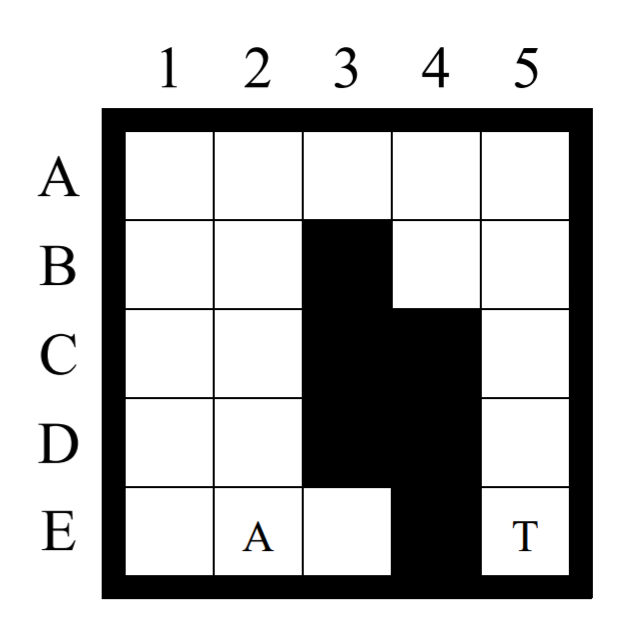
\includegraphics[width=0.35\linewidth]{Report/Part1/maze.PNG}  
\caption{Sample maze problem}
\label{samplemaze}
\end{figure}

In \emph{figure \ref{samplemaze}} we can see a small sample maze. Our initial state is cell \emph{E2} and our goal state is \emph{E5}. Our agent does not initially know about the walls so we will walk through what happens that causes the agent to first move to cell \emph{E3}.
\begin{enumerate}
  \item Begin in \emph{E2} and check for walls. No adjacent walls exist, so perform $A^* search$
    \begin{itemize}
    \item Add E2 to open list
    \item Remove node in open list with lowest f-value (E2) and add to closed list. Then add neighbors to open list
        \begin{itemize}
            \item Cell E3: g(n) = 1, h(n) = 2, f(n) = 3 
            \item Cell D2: g(n) = 1, h(n) = 4, f(n) = 5 
            \item Cell E1: g(n) = 1, h(n) = 4, f(n) = 5 
        \end{itemize}
        \item Remove node in open list with lowest f-value (E3) and add to closed list. Then add neighbors to open list. (We do not add a node that is in the closed list)
        \begin{itemize}
            \item Cell E4: g(n) = 2, h(n) = 1, f(n) = 3 
            \item Cell D3: g(n) = 2, h(n) = 3, f(n) = 5
            \item Cell D2: g(n) = 1, h(n) = 4, f(n) = 5 
            \item Cell E1: g(n) = 1, h(n) = 4, f(n) = 5 
        \end{itemize}
        \item Remove node in open list with lowest f-value (E4) and add to closed list. Then add neighbors to open list.
        \begin{itemize}
            \item Cell E5: g(n) = 3, h(n) = 0, f(n) = 3
            \item Cell D4: g(n) = 3, h(n) = 2, f(n) = 5
            \item Cell D3: g(n) = 2, h(n) = 3, f(n) = 5
            \item Cell D2: g(n) = 1, h(n) = 4, f(n) = 5 
            \item Cell E1: g(n) = 1, h(n) = 4, f(n) = 5
        \end{itemize}
        \item Remove node in open list with lowest f-value (E5) and this is our goal node. $A^* search$ is now complete, and has returned the path: $E2 \longrightarrow E3 \longrightarrow E4 \longrightarrow E5$
    \end{itemize}
    \item Now we move along this path to E3, and realize a wall exists in our path (E4). We then perform another \emph{$A^*$ search}.
\end{enumerate}
The above walk through demonstrates why our agent will move east as its first action. It is inherently because the agent cannot observe the walls that are in its way until it is adjacent to the walls. This causes the \emph{$A^*$ search} to find the optimal path without considering the blockage.


It is important to note that in searching these finite grid worlds, we are guaranteed to either find a solution if it exists. And if a solution does not exist, we know that this is the case. The reason behind this is that all cells in our grid world are connected, with some being walls. We can think of these walls as discontinuations in the grid. Because of this, any location in our grid that is not an island can be reached in some form or another through a linked list of cells travelled. On the other hand, any islands that exist cannot be reached from other islands. This is very analogous to the earth, if we assume water represents our walls in the grid. We can technically get to any point on a connected piece of land by car, but not so if the land is surrounded by water. This is automatically implemented in \emph{$A^*$ search} since any nodes in our open list can be traced to the initial start node. After all nodes are in the closed list, our open list becomes empty  and the goal is not reached, we know that no solution exists. And this can be done in finite time since our grid world is finite to begin with.

We can also analyze the maximum number of cells an agent would travel before it reaches its goal or finds out it cannot reach the goal. Take the same 5 X 5 grid in \emph{figure \ref{samplemaze}}. We will prove the following:


\begin{qoute}
\emph{Prove that the number of moves of the agent until it reaches the target or discovers that this is impossible is bounded from above by the number of unblocked cells squared.}
\end{qoute}
\begin{proof}
Let $S$ be the set of all cells in the grid, with $|S| = 25$ and $B$ be the set of all unblocked cells for the known environment, where $|B| = 19$. By using $A^* search$, we will be adding each expanded node to the closed list, meaning for node x, $\forall x \in closedList:$ $x \notin openList$. Therefore, the set of all moves, $X$, has the property that $|X| \leq |B|$.


This shows that for a known environment, the number of moves the agent can explore until it reaches the goal cannot be greater than the state space. However, we are dealing with an initially unknown environment.We must therefore expand this definition for \emph{repeated forward/backward $A^* search$}. The pseudo code of this is shown below:

\begin{algorithm}
    \caption{Repeated forward/backward $A^* search$}
    \begin{algorithmic}
    
    \STATE $current = start$
    \STATE $path \leftarrow computeAstar(current)$
    \WHILE{$current \neq goal$}
    \STATE $walls \leftarrow update()$
    \IF{$path.next \neq wall$}
        \STATE $current \leftarrow path.next$
    \ELSE
        \STATE $path \leftarrow computeAstar(current, walls)$
        \IF{$path == NULL$}
            \RETURN{"No Path Exists!"}
        \ENDIF
    \ENDIF
    \ENDWHILE
    \end{algorithmic}
\end{algorithm}

We can observe that \emph{Repeated forward/backward $A^* search$} has the only difference with the fact that it calls $A^* search$ every time it encounters a new obstacle on its current path. Therefore, since each $A^* search$ is bounded by $|X| \leq |B|$, where $X$ is the set of all nodes explored by $A^* search$ and $B$ is the set of all open cells on the grid, we can also infer that $A^* search$ will not be called on nodes that have already been travelled, since we have a static environment. Therefore, for the set of travelled nodes, $Z$, we have $|Z| \leq |X|*m$, where $m$ is the amount of times $A^* search$ is called. And we know from before, that $m \leq |X|$. We can assume a worst case situation and have $m = |X|$. Finally, by substitution we obtain $|Z| \leq |X|^2$ and the upper bound of this with substitution would be $|Z| \leq |B|^2$.

\end{proof}
%!TEX root =  ../Report.tex

\section{Part 2: The Effects of Ties}                               
\label{sec: Part 2}

In previous sections, it was mentioned that $A^*$ \emph{search} is an informed search algorithm, and therefore uses an evaluation function, denoted as $f(n) = g(n) + h(n)$. In this function, $g(n)$ is the traveled distance from node $n$ to the initial state, and $h(n)$ is the heuristic function. In our priority queue, we will be prioritizing nodes with the smallest $f(n)$ value, but the problem is that multiple nodes can have the same $f(n)$ value. So what do we do if the smallest $f(n)$ value happens to be in a tie with 1 or more other nodes? 


We will look at the run times for breaking this tie by prioritizing the nodes with the superior $g(n)$ value. In particular, we will implement this through our \texttt{Node} class, by using this line for prioritizing nodes with a larger $g(n)$:
\begin{lstlisting}
    return self.g >= otherNode.g #tie breaker for larger g value
\end{lstlisting}

and changing this line to the following for prioritizing smaller $g(n)$ values:

\begin{lstlisting}
    return self.g < otherNode.g #tie breaker for smaller g value
\end{lstlisting}

The way this works is that the \texttt{heapq} library makes comparisons for each item it has by using the \texttt{<} operator. When two $f(n)$ values are the same, we defined this in our \texttt{Node} class and it will go to the line above and choose either the node with the larger or smaller $g(n)$ value. Below are the results.

\begin{figure}[H]
  \centering
  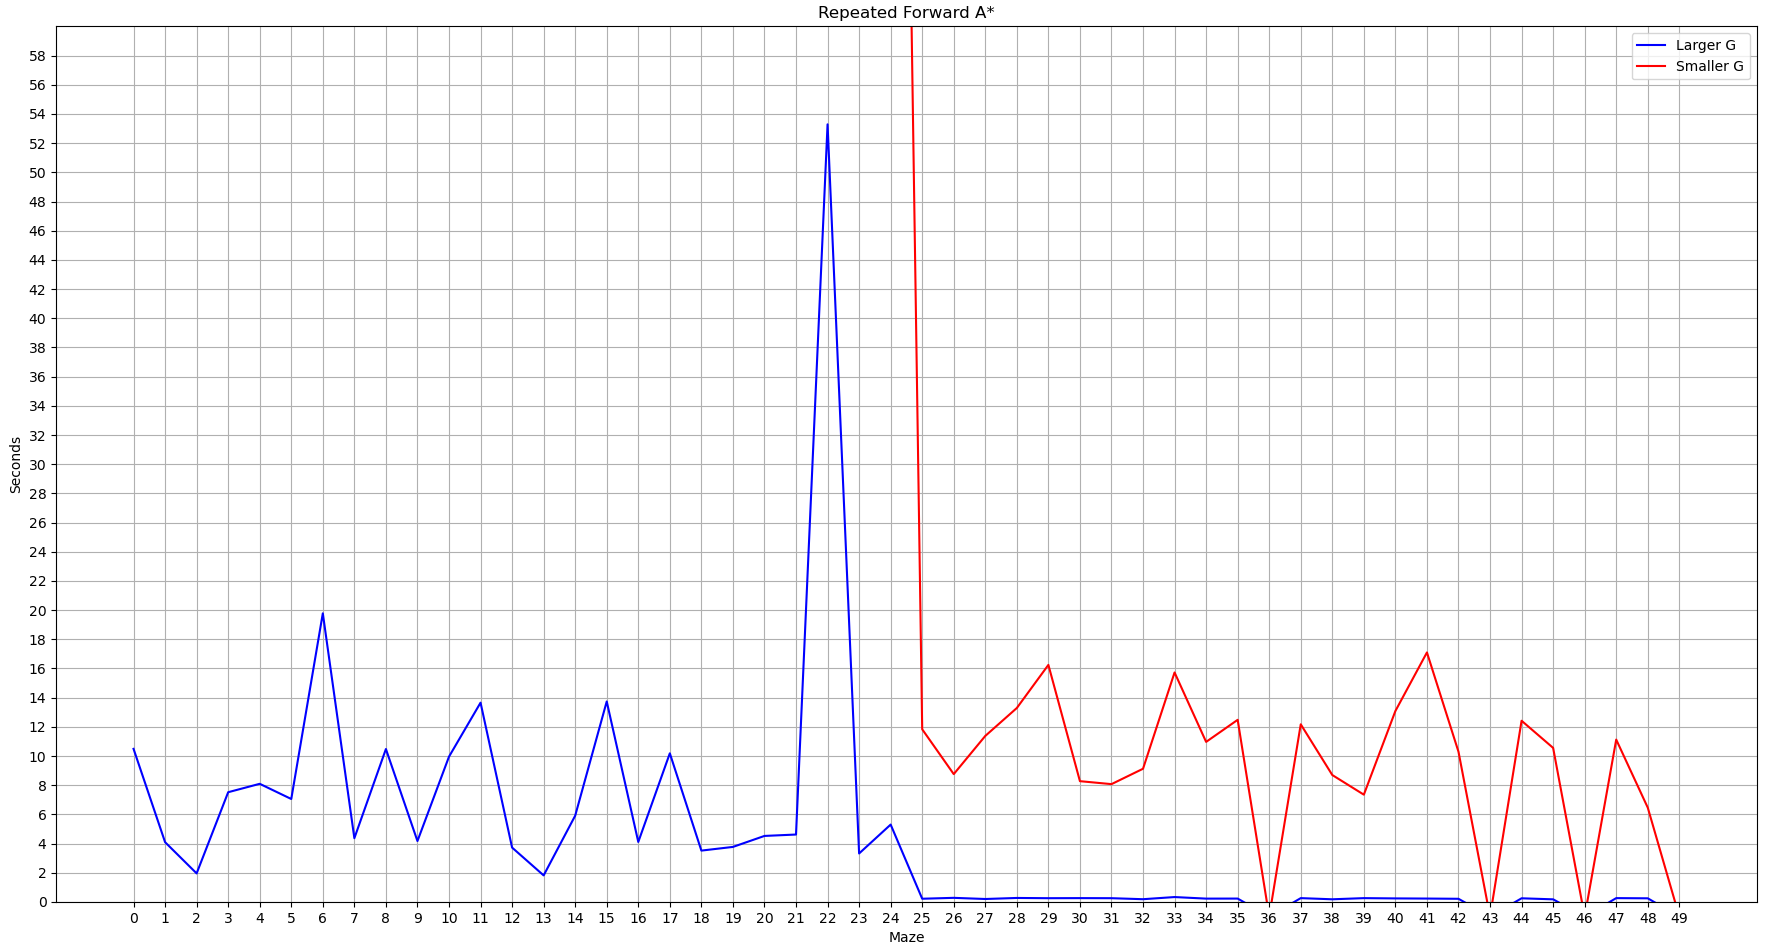
\includegraphics[width=1\linewidth]{Report/Part2/Figure_1.png}  
\caption{Repeated Forward $A^*$ $f(n)$ tie-breaker comparison}
\end{figure}

In the test, mazes 0-24 were the backtracked mazes and mazes 25-49 were the random mazes. It can be seen that choosing the smaller $g(n)$ value results in considerably longer run times, to the point where in our backtracked mazes it was taking upwards of 200 seconds (outside the range of this graph). It is also important to note that for mazes where the run time is at 0, it is because the solution was not found. This means either the start or goal node was blocked off by walls.


Our results show that using a larger $g(n)$ value as the tie breaker performs significantly better than using a smaller $g(n)$ value, and we will now explore the reason for this. 


Lets assume we run $A^*$ \emph{search} on the graph below, where $A1$ is our start and $E5$ is our goal. Heuristic values are shown in each cell.

\begin{figure}[H]
  \centering
  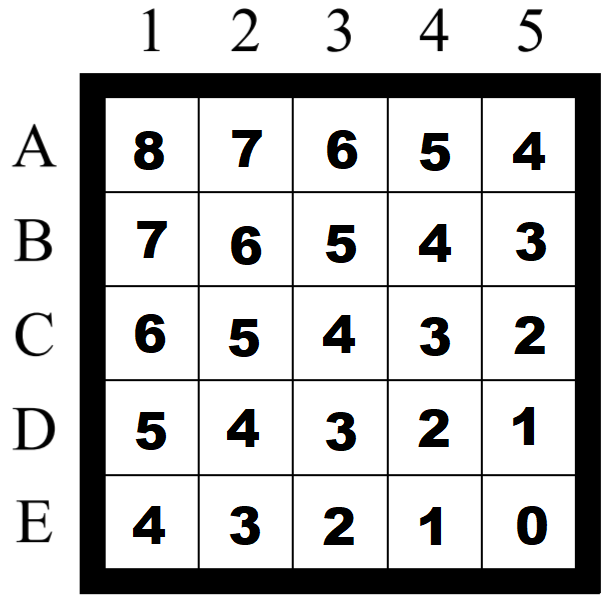
\includegraphics[width=0.31\linewidth]{Report/Part2/g tie breaker/samplegraph.png}  
\caption{Sample maze}
\end{figure}

We will first begin with an $A^*$ \emph{search} where the larger $g(n)$ is favored.
\linebreak
\begin{figure}[H]
\begin{subfigure}[b]{.3\textwidth}
  \centering
  \includegraphics[width=0.95\linewidth]{Report/Part2/g tie breaker/larger g/1.png}  
\end{subfigure}
\begin{subfigure}[b]{.3\textwidth}
  \centering
  \includegraphics[width=0.95\linewidth]{Report/Part2/g tie breaker/larger g/2.png}  
\end{subfigure}
\begin{subfigure}[b]{.3\textwidth}
  \centering
  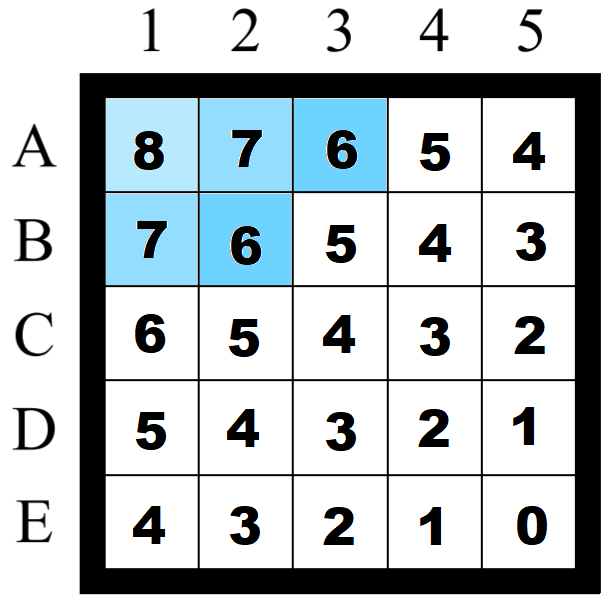
\includegraphics[width=0.95\linewidth]{Report/Part2/g tie breaker/larger g/3.png}  
\end{subfigure}
\newline
\linebreak
\begin{subfigure}[b]{.3\textwidth}
  \centering
  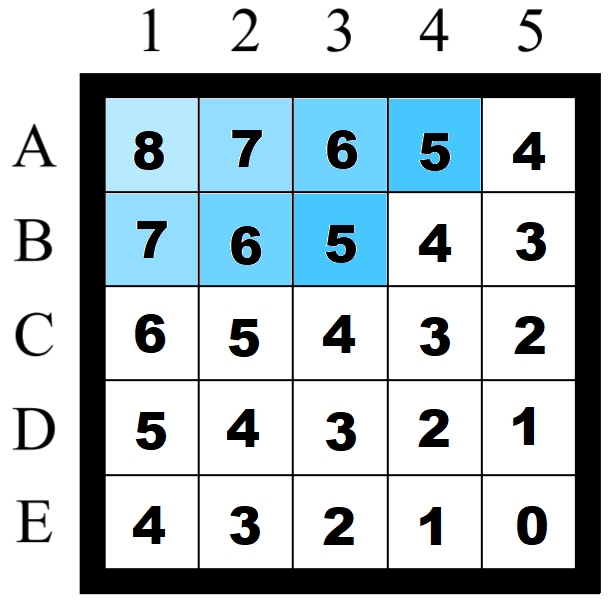
\includegraphics[width=0.95\linewidth]{Report/Part2/g tie breaker/larger g/4.png}  
\end{subfigure}
\begin{subfigure}[b]{.3\textwidth}
  \centering
  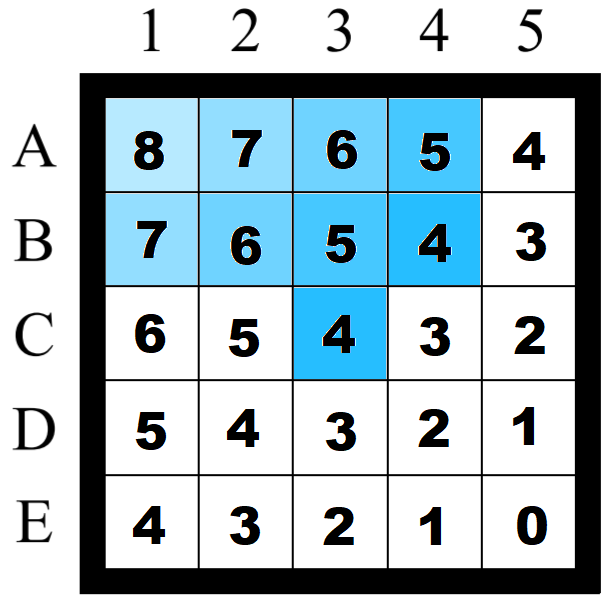
\includegraphics[width=0.95\linewidth]{Report/Part2/g tie breaker/larger g/5.png}  
\end{subfigure}
\begin{subfigure}[b]{.3\textwidth}
  \centering
  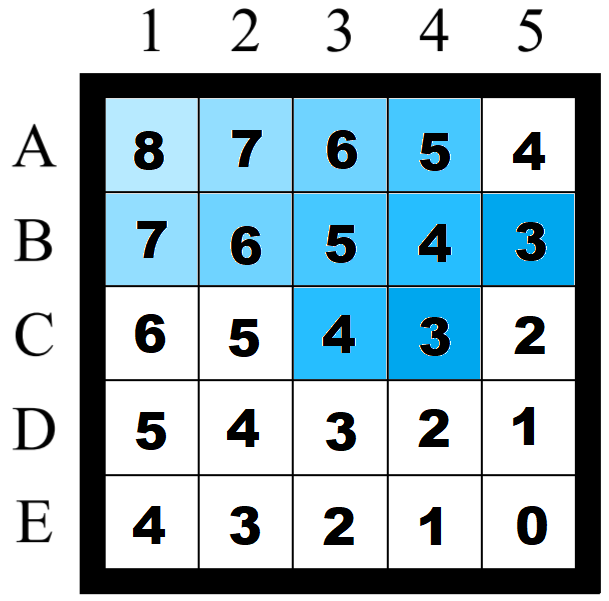
\includegraphics[width=0.95\linewidth]{Report/Part2/g tie breaker/larger g/6.png}  
\end{subfigure}
\newline
\linebreak
\begin{subfigure}[b]{.3\textwidth}
  \centering
  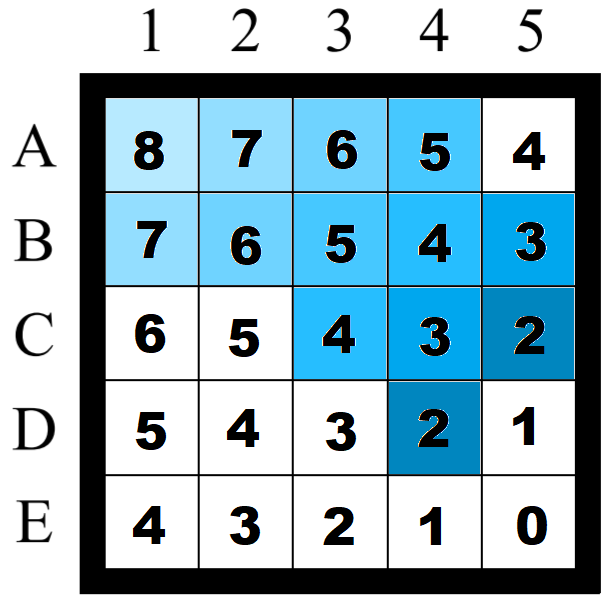
\includegraphics[width=0.95\linewidth]{Report/Part2/g tie breaker/larger g/7.png}  
\end{subfigure}
\begin{subfigure}[b]{.3\textwidth}
  \centering
  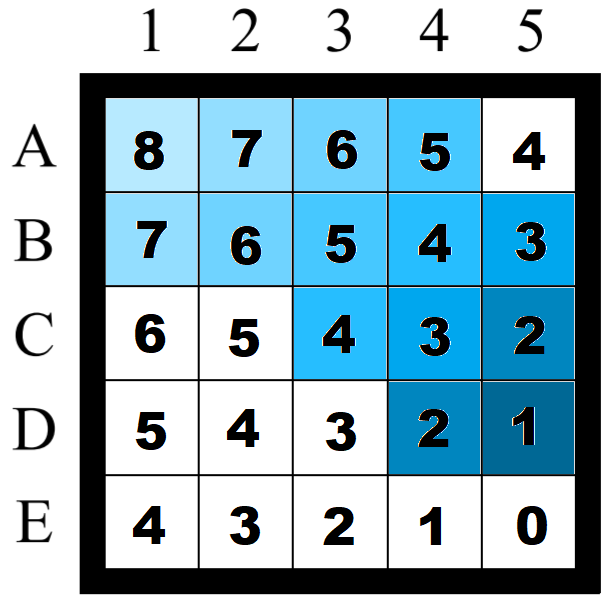
\includegraphics[width=0.95\linewidth]{Report/Part2/g tie breaker/larger g/8.png}  
\end{subfigure}
\begin{subfigure}[b]{.3\textwidth}
  \centering
  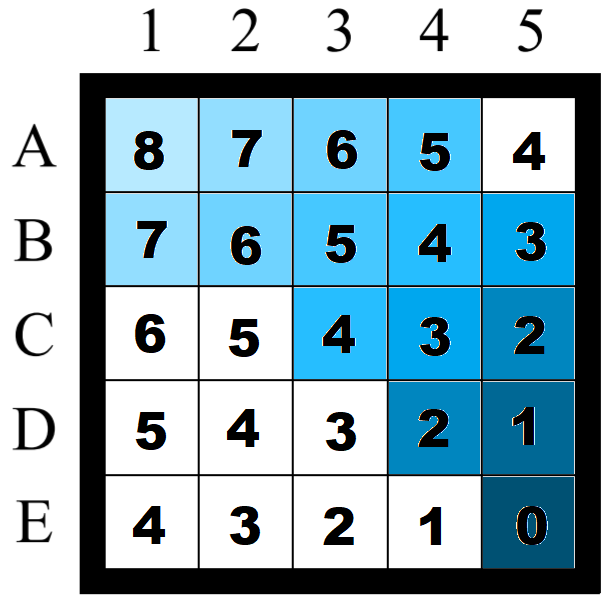
\includegraphics[width=0.95\linewidth]{Report/Part2/g tie breaker/larger g/9.png}  
\end{subfigure}


\caption{Forward $A*$ larger $g(n)$}
\end{figure}

As we observe, the solution is found in iteration 9 of the search. For each node expanded, the $f(n)$ value is actually always the same, since no obstacles exist and each step has a cost of 1. Therefore, we expand the nodes with the largest distance from the start node, since those have the largest $g(n)$ values.


Now lets look at the run through of {Forward $A^*$} which prioritizes a smaller $g(n)$.
\linebreak
\begin{figure}[H]
\begin{subfigure}[b]{.3\textwidth}
  \centering
  \includegraphics[width=0.95\linewidth]{Report/Part2/g tie breaker/smaller g/1.png}  
\end{subfigure}
\begin{subfigure}[b]{.3\textwidth}
  \centering
  \includegraphics[width=0.95\linewidth]{Report/Part2/g tie breaker/smaller g/2.png}  
\end{subfigure}
\begin{subfigure}[b]{.3\textwidth}
  \centering
  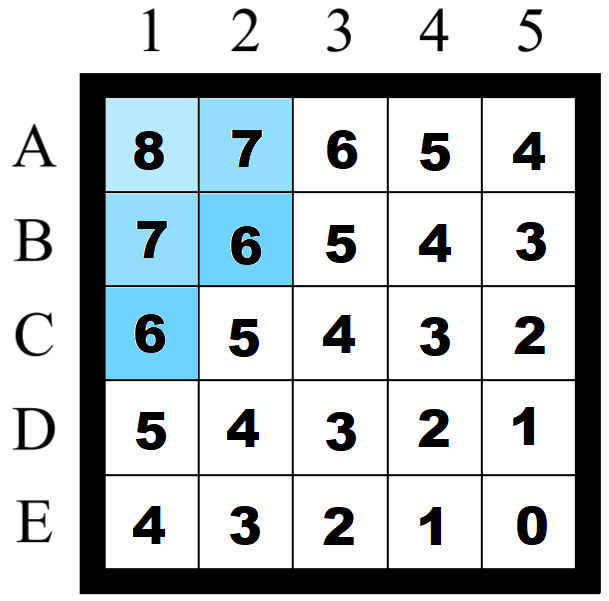
\includegraphics[width=0.95\linewidth]{Report/Part2/g tie breaker/smaller g/3.png}  
\end{subfigure}
\newline
\linebreak
\begin{subfigure}[b]{.3\textwidth}
  \centering
  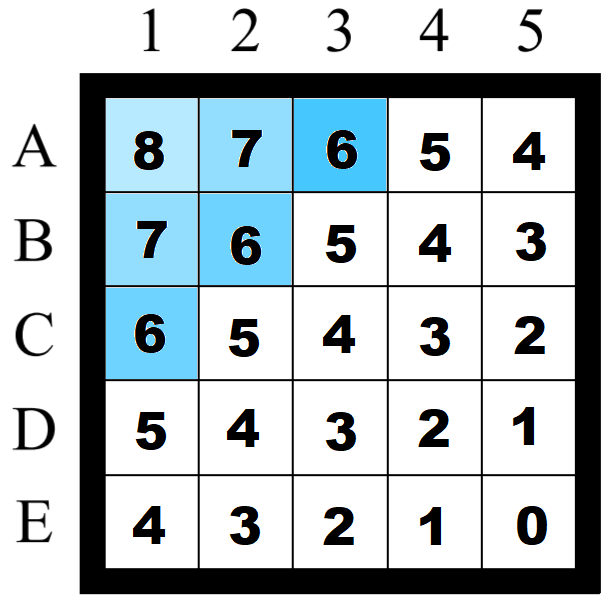
\includegraphics[width=0.95\linewidth]{Report/Part2/g tie breaker/smaller g/4.png}  
\end{subfigure}
\begin{subfigure}[b]{.3\textwidth}
  \centering
  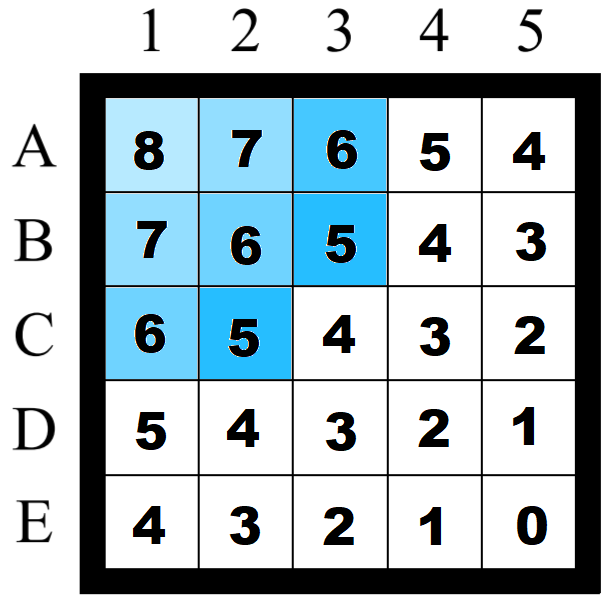
\includegraphics[width=0.95\linewidth]{Report/Part2/g tie breaker/smaller g/5.png}  
\end{subfigure}
\begin{subfigure}[b]{.3\textwidth}
  \centering
  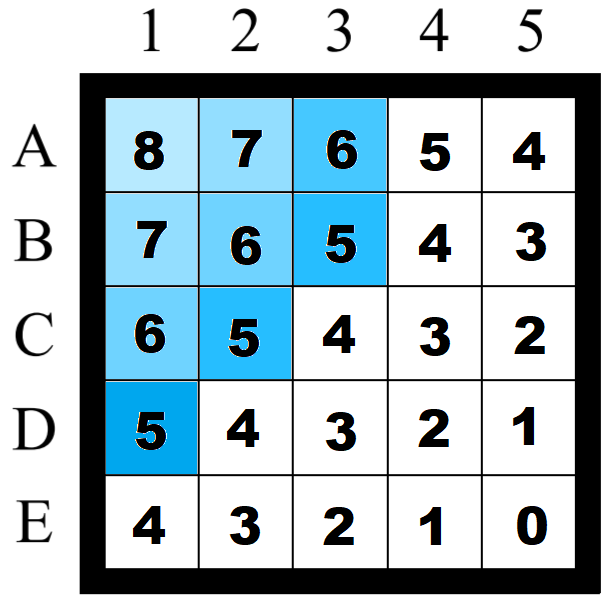
\includegraphics[width=0.95\linewidth]{Report/Part2/g tie breaker/smaller g/6.png}  
\end{subfigure}
\newline
\linebreak
\begin{subfigure}[b]{.3\textwidth}
  \centering
  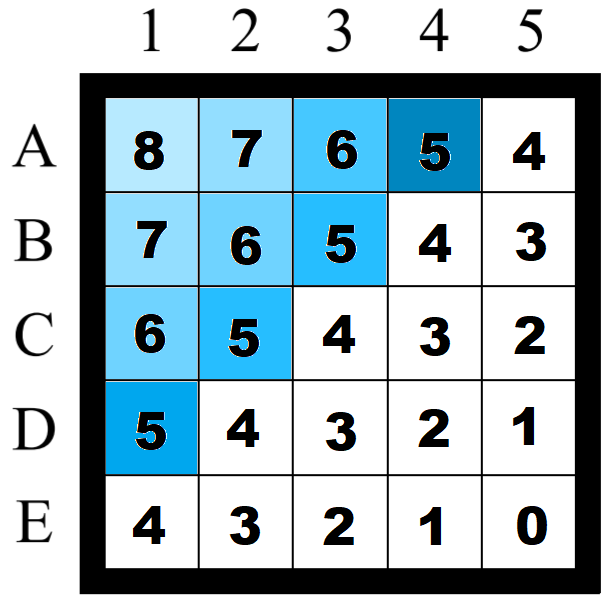
\includegraphics[width=0.95\linewidth]{Report/Part2/g tie breaker/smaller g/7.png}  
\end{subfigure}
\begin{subfigure}[b]{.3\textwidth}
  \centering
  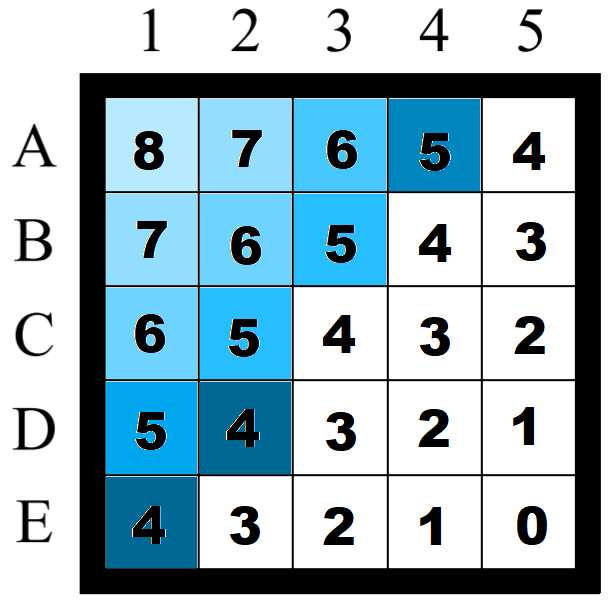
\includegraphics[width=0.95\linewidth]{Report/Part2/g tie breaker/smaller g/8.png}  
\end{subfigure}
\begin{subfigure}[b]{.3\textwidth}
  \centering
  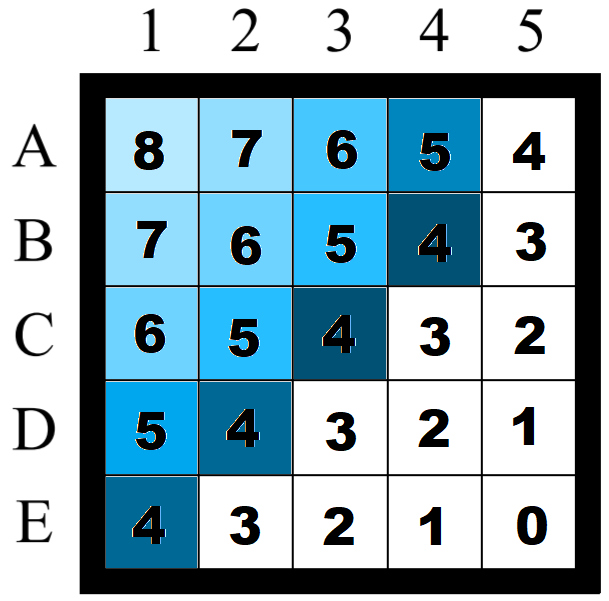
\includegraphics[width=0.95\linewidth]{Report/Part2/g tie breaker/smaller g/9.png}  
\end{subfigure}


\caption{Forward $A*$ smaller $g(n)$}
\end{figure}

In the results we see that by iteration 9, we have not reached the goal. In fact, it only seems that half of the map has been explored. So why is this the case? Logically, this is because each node inherently has the same $f(n)$ value, once again, because of there being no obstacles, and the cost of each step being 1. Therefore, the priority is on the nodes closest to the start.


But there is a deeper meaning behind choosing the larger or smaller $g(n)$ value in this situation. If we re-examine the above to tests, we notice something. It is that for the iterations where the larger $g(n)$ value is favored, $A^*$ \emph{search} acts the same as \emph{Depth First Search}. And on the other-hand, for the iterations where the smaller $g(n)$ value is favored, $A^*$ \emph{search} acts the same as \emph{Breadth First Search}. This is not a coincidence though. In fact, due to the layout of this graph (where each step gets us further away from the start and closer to the goal), you could think that the evaluation function of these 2 algorithms is defined as $f(n) = g(n)$, and \emph{Depth First Search} has a priority queue where a larger $f(n)$ is prioritized, and \emph{Breadth First Search} has a priority queue where a smaller $f(n)$ is prioritized. But how does this relate to $A^*$ \emph{search}? Well as mentioned before, for this environment and search problem, our $f(n)$ value remains the same for each visited node, therefore, by choosing to break the tie with the value of $g(n)$, we are inherently just letting $f(n) = g(n)$, and altering the priority queue from a normal queue and a stack by choosing if a smaller or larger $g(n)$ value is prioritized.

\begin{figure}[ht]
\begin{subfigure}{.5\textwidth}
  \centering
  \includegraphics[width=0.8\linewidth]{Report/Part2/larger_g_forward_302.png}  
  \caption{Larger $g(n)$, 302 nodes path length}
\end{subfigure}
\begin{subfigure}{.5\textwidth}
  \centering
  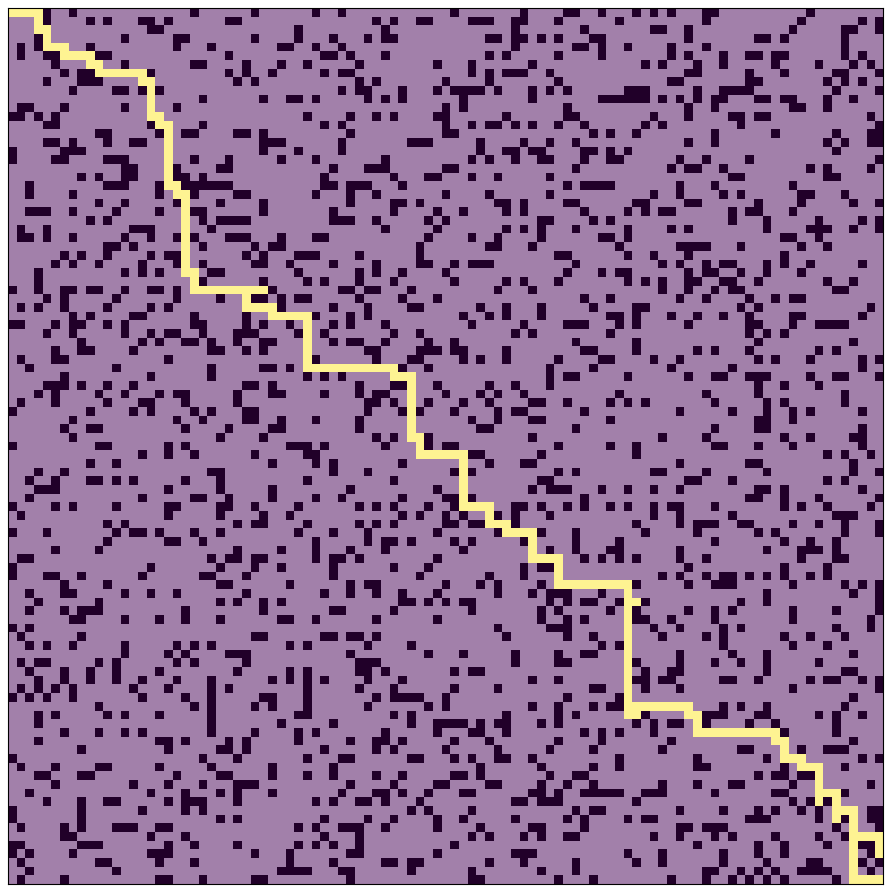
\includegraphics[width=0.8\linewidth]{Report/Part2/smaller_g_forward_260.png}  
  \caption{Smaller $g(n)$, 260 nodes path length}
\end{subfigure}
\newline
\linebreak
\linebreak
\begin{subfigure}{.5\textwidth}
  \centering
  \includegraphics[width=0.8\linewidth]{Report/Part2/larger_g_forward_3178.png}  
  \caption{Larger $g(n)$, 3178 nodes path length}
\end{subfigure}
\begin{subfigure}{.5\textwidth}
  \centering
  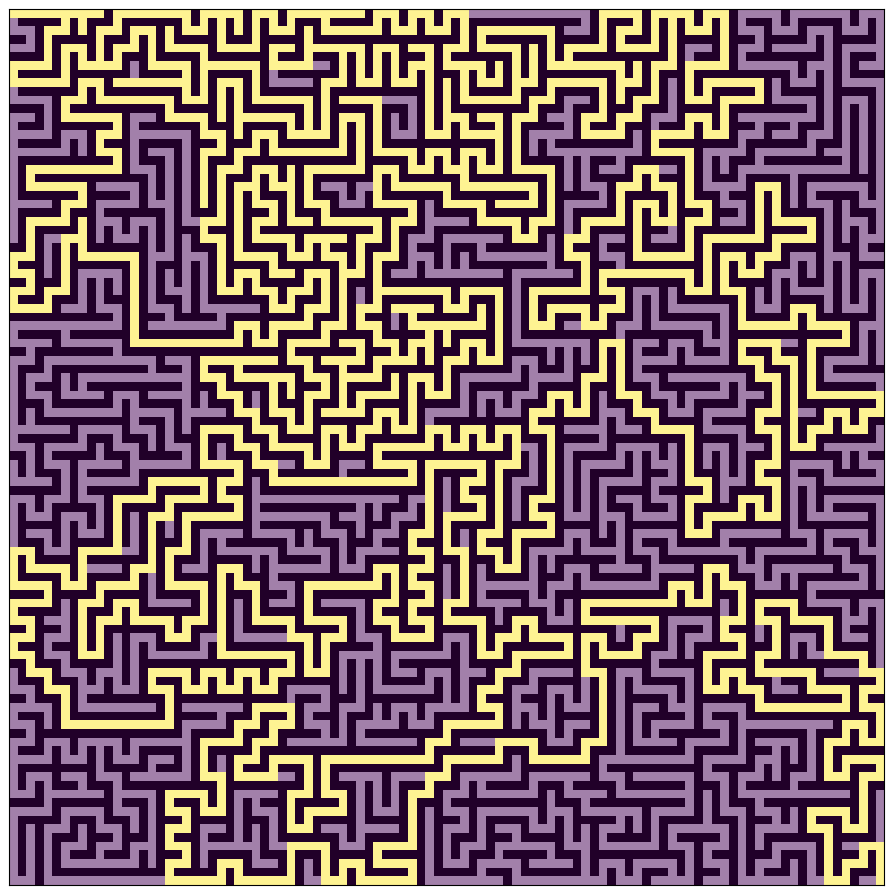
\includegraphics[width=0.8\linewidth]{Report/Part2/smaller_g_forward_4846.png}  
  \caption{Smaller $g(n)$, 4846 nodes path length}
\end{subfigure}
\caption{Repeated Forward $A^*$ tie-breaker comparison with different mazes}
\end{figure}

\section{Part 3: Forward vs. Backward }
\label{sec: Part 2}

Previously, we examined how tie breaking for the same $f(n)$ value with the $g(n)$ value can lead to drastic differences in run times for \emph{Repeated Forward $A^*$ search}. In this section we will examine another variation in the \emph{$A^*$ search} algorithm.


Up to now, we have been examining \emph{Repeated Forward $A^*$ search}, where the path is planned starting from the agent to the goal. However, a variation, called \emph{Repeated Backward $A^*$ search} exists, which means that the path is planned from the goal to the agent, and then executed by the agent. Every time a new obstacle is in the path, the algorithm computes a new path from the goal to the agent. Below are the run times of comparing the two methods. In our tests, we consider a larger $g(n)$ value as the tie breaker, and after that, which ever node was placed first in the priority queue.

\begin{figure}[H]
  \centering
  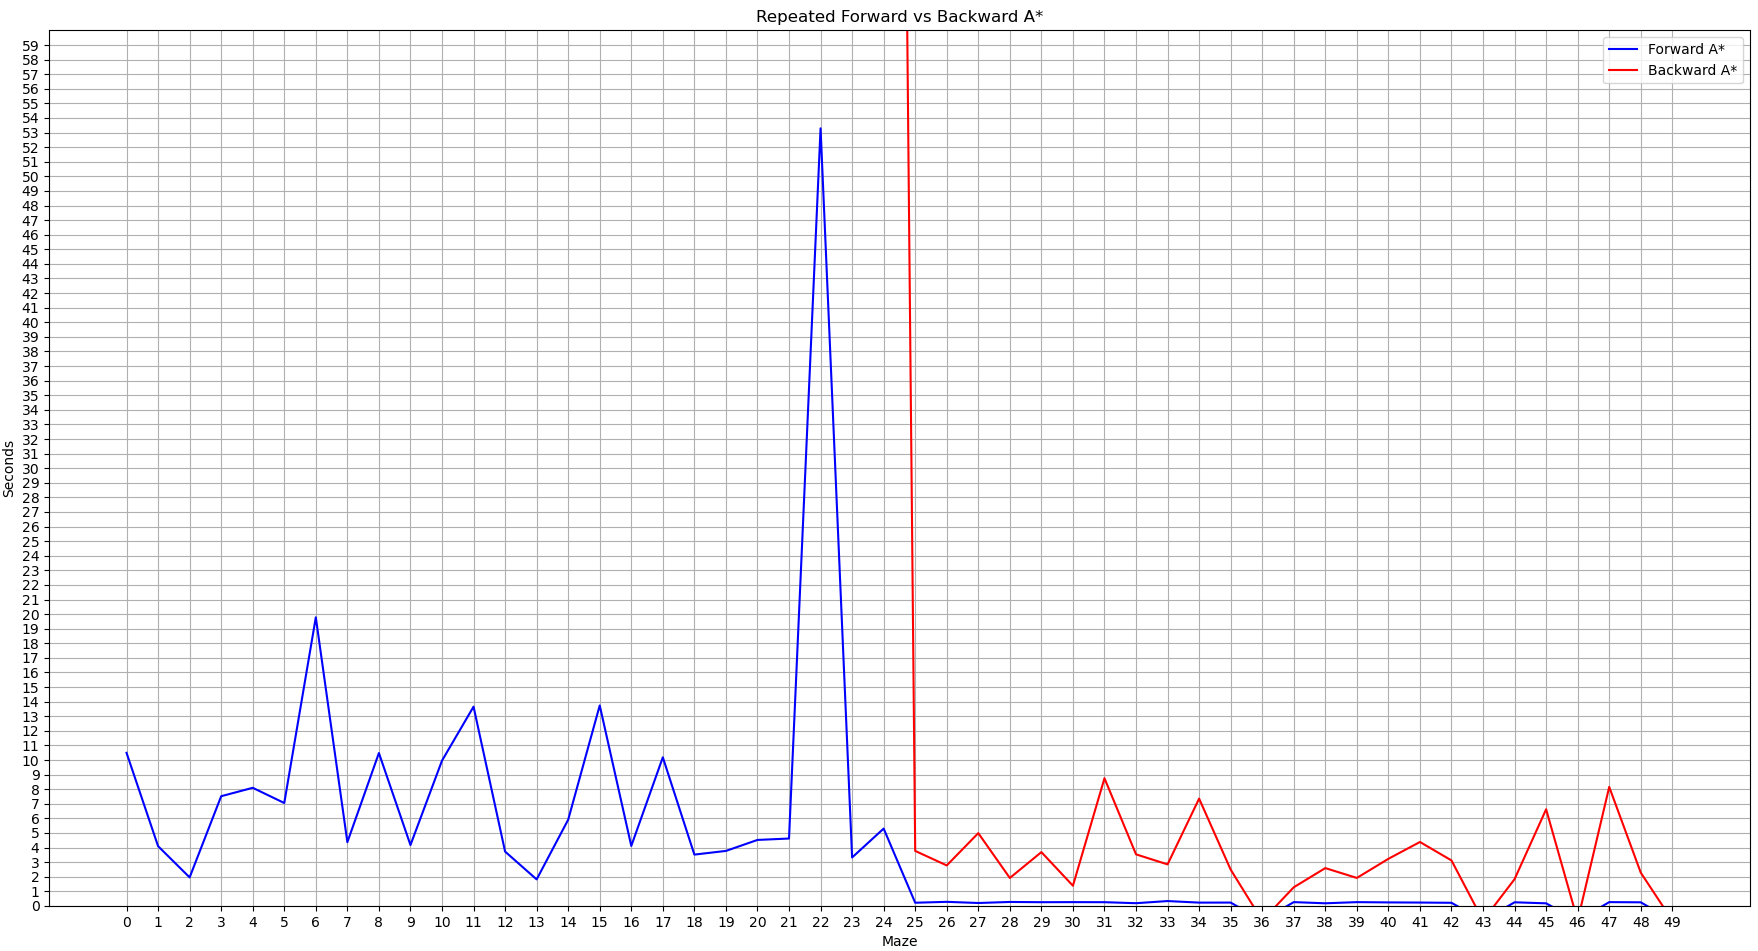
\includegraphics[width=1\linewidth]{Report/Part3/Figure_2.png}  
\caption{Repeated Forward vs Backward $A^*$ Comparison}
\end{figure}

Our results show that \emph{Repeated Backward $A^*$} performed significantly worst than \emph{Repeated Forward $A^*$}. For our backtracked mazes, the run times of \emph{Repeated Forward $A^*$} even surpassed 60 seconds, often over 200 seconds.


The reason for the long run times of \emph{Repeated Backward $A^*$} has to do with an observation we previously made. We saw in \emph{Figure 6} that as long as we have an open map and our start and goal are placed in a certain way (the same start and goal is chosen for all our tests), \emph{$A^*$ search} will act as a \emph{Depth First Search}. This was because all cells would have the same $f(n)$ value. However, in our mazes this is not the case. We have many walls, and therefore, $f(n)$ will alter for paths to many cells. 


Now how does this relate to the run times of Forward and Backward \emph{$A^*$ search}? In \emph{Repeated Forward $A^*$}, we perform a \emph{Depth First Search} from the start to the goal. As we move along and encounter walls, we recompute the path, and we will hit the wall very early in our search. This means all cells visited after passing the wall will all have the same $f(n)$ value and the rest of the algorithm will follow \emph{Figure 6}.


On the other hand, with \emph{Repeated Backward $A^*$} we will be computing a path from the goal to the start. This means after our first iteration, we will move until we meet a wall. Then, in our new computation of the path, our algorithm will compute a \emph{Depth First Search} until it meets the wall. Now here lies the problem. Since our \emph{Depth First Search} is from the goal to the start, and the wall is near our start, there are many nodes in our priority queue with smaller $f(n)$ values than the node that goes around the wall. So now, we must expand all of those nodes first, and then continue with the final path. 


\begin{figure}[H]
\begin{subfigure}{.5\textwidth}
  \centering
  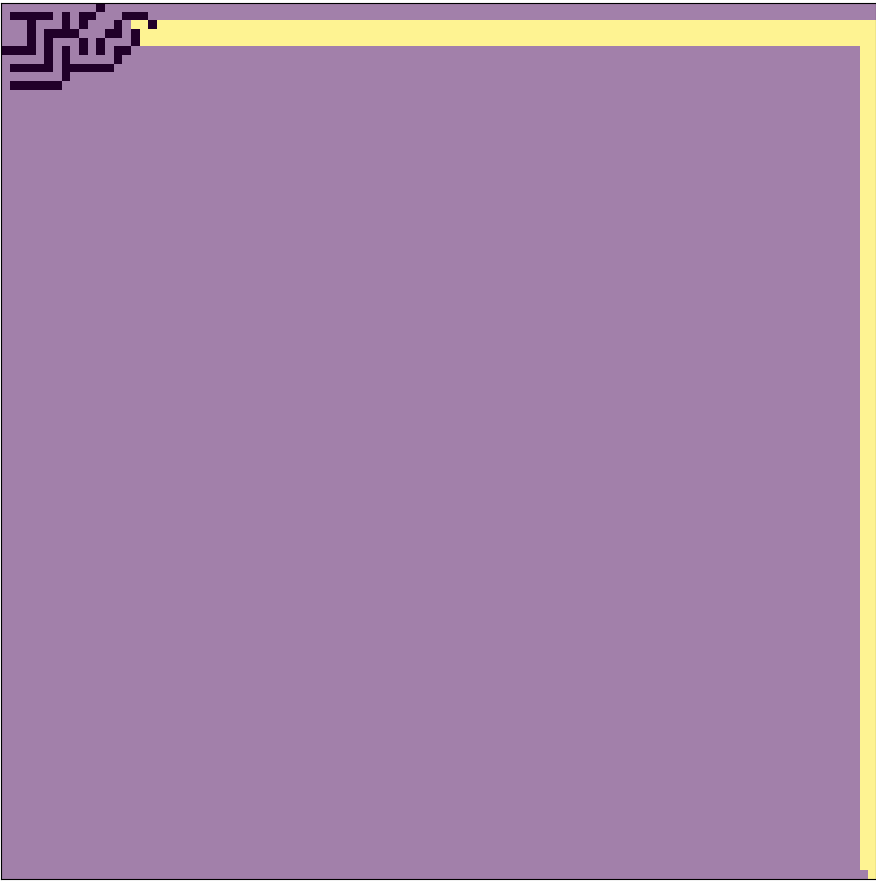
\includegraphics[width=0.8\linewidth]{Report/Part3/Forward_Astar_iter21.png}  
  \caption{Forward \emph{$A^*$ search}}
\end{subfigure}
\begin{subfigure}{.5\textwidth}
  \centering
  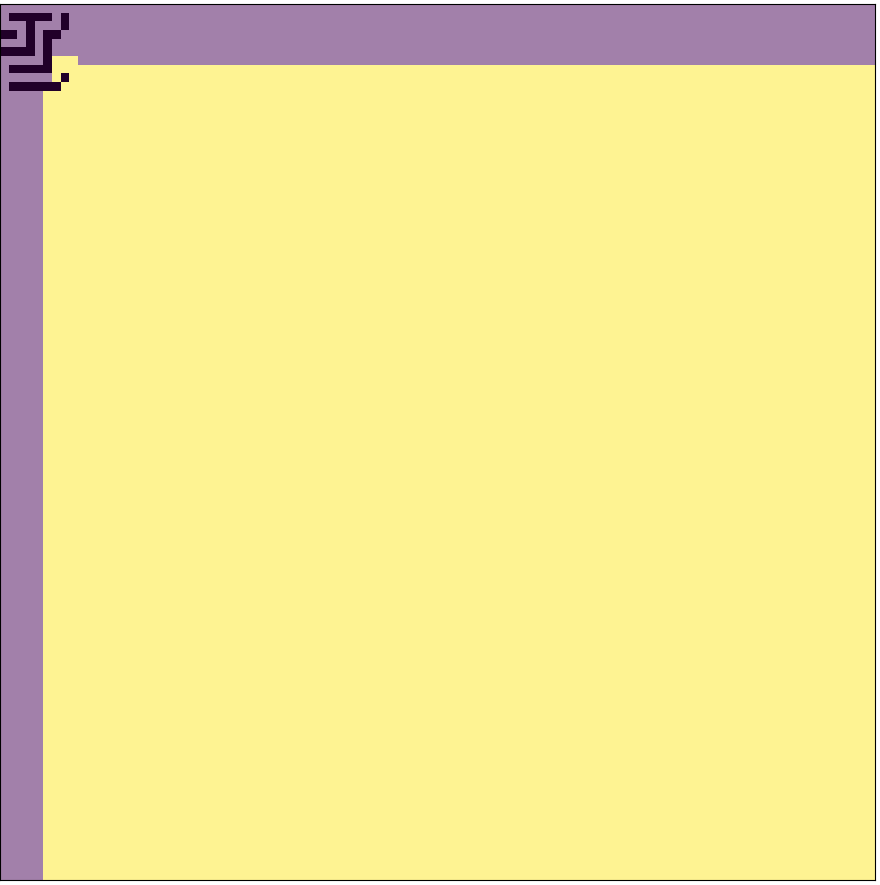
\includegraphics[width=0.8\linewidth]{Report/Part3/Backward_Astar_iter21.png}  
  \caption{Backward \emph{$A^*$ search}}
\end{subfigure}
\caption{The visited nodes of an iteration of $A^* search$}
\end{figure}


In essence, both variants of \emph{$A^*$ search} are actually the same. The only difference is where in our first \emph{Depth First Search} path the wall is located. The further the wall is located down the initial \emph{Depth First Search} path, will mean our search will take much longer then if we had reversed order. In general, you could think of it as the midpoint of the initial expanded path. If the obstacle is past one side of the path, \emph{Repeated Backward $A^*$} is better. And if the obstacle is on the other side of the midpoint, \emph{Repeated Forward $A^*$} will perform better.

\begin{figure}[H]
\begin{subfigure}{.5\textwidth}
  \centering
  \includegraphics[width=0.8\linewidth]{Report/Part3/larger_g_forward_302.png}  
  \caption{Forward $A^*$, 302 nodes path length}
\end{subfigure}
\begin{subfigure}{.5\textwidth}
  \centering
  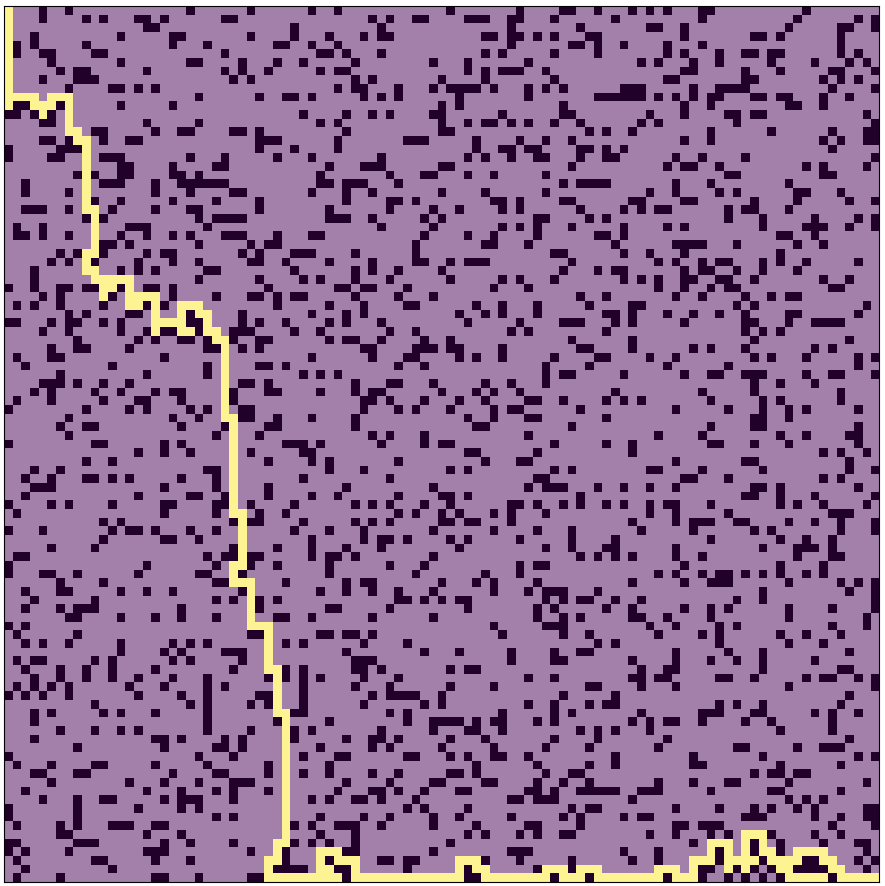
\includegraphics[width=0.8\linewidth]{Report/Part3/larger_g_backward_339.png}  
  \caption{Backward $A^*$, 339 nodes path length}
\end{subfigure}
\newline
\linebreak
\linebreak
\begin{subfigure}{.5\textwidth}
  \centering
  \includegraphics[width=0.8\linewidth]{Report/Part3/larger_g_forward_3178.png}  
  \caption{Forward $A^*$, 3178 nodes path length}
\end{subfigure}
\begin{subfigure}{.5\textwidth}
  \centering
  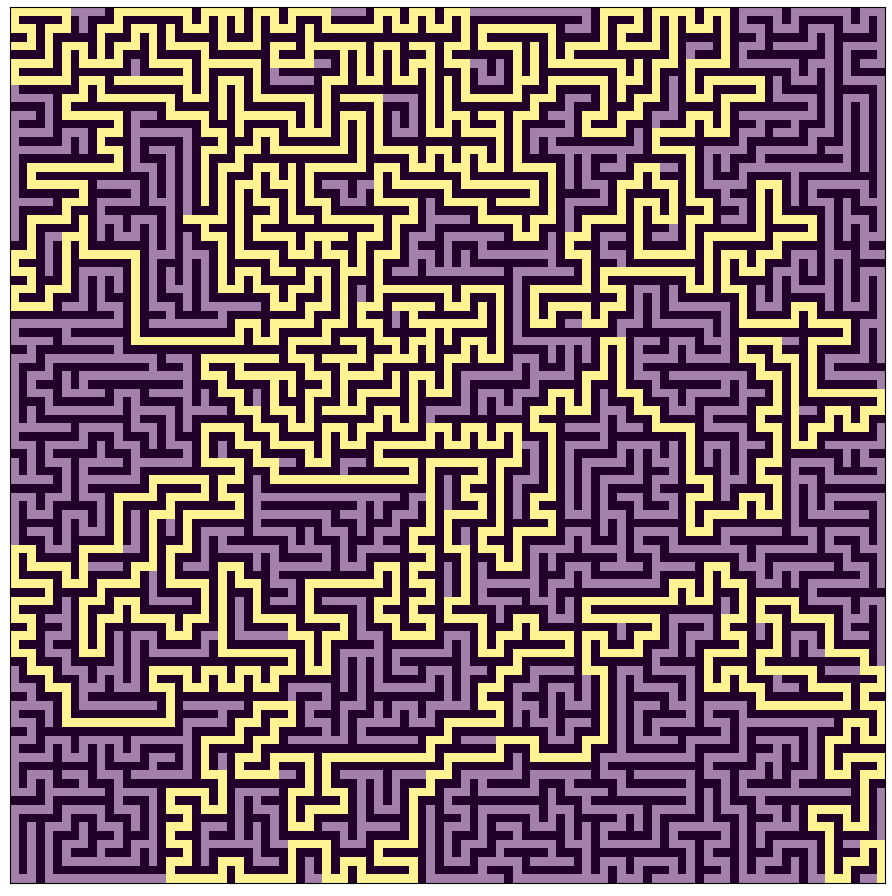
\includegraphics[width=0.8\linewidth]{Report/Part3/larger_g_backward_4861.png}  
  \caption{Backward $A^*$, 4861 nodes path length}
\end{subfigure}
\caption{Repeated Forward vs Backward $A^*$ comparison with different mazes}
\end{figure}
\section{Part 4: Heuristics in the Adaptive A* }
\label{sec: Part 4}

In our grid world, we are operating with an atomic unit where each cell is the atom. In our grid world, we can only move in the main compass directions of north, south, west, and east. This means that the shortest distance between two cells is always the $Manhattan Distance$. This simply means that if we have 2 points, $p_1(x_1,y_1)$ and $p_2(x_2,y_2)$, then the Manhattan Distance between them is given by  $D = |x_2 - x_1| + |y_2 - y_1|$. 


In order for \emph{$A^*$ search} to work properly, it requires a consistent heuristic. A consistent heuristic is defined as one that has the distance from the current node to the goal as always less than or equal to distance from any neighbor node to the goal plus the distance to reach that neighbor. In other words, assume $n$ is any node on the grid, then $h(n) \leq c(n,p) + h(p)$, where $h(n)$ is our heuristic value of node $n$, $c(n,p)$ is the distance from node $n$ to one other node $p$, and $h(p)$ is the heuristic value of node $p$. Of course, using simple geometry, this must always be true when dealing with euclidean distances, as shown below.
\begin{figure}[H]
  \centering
  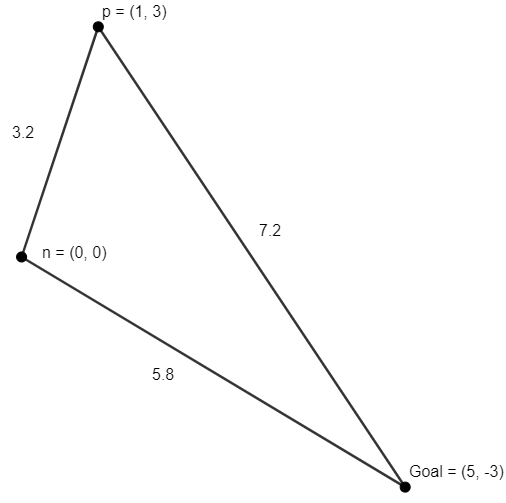
\includegraphics[width=0.5\linewidth]{Report/Part4/Annotation 2020-07-10 224338.png}  
\caption{Consistent heuristics with Euclidean Distance}
\end{figure}

We can observe that the heuristic above is admissible since $h(n) \leq c(n,p) + h(p)$ holds. In other words, $5.8 \leq 3.2 + 7.2$ due to the triangle inequality. Namely, it is impossible to have a triangle where the length of the sum of 2 sides is larger than the third side. Now we will prove this for the case of Manhattan Distances.


\linebreak
\begin{qoute}
\emph{Prove that Manhattan distances are consistent in
grid worlds in which the agent can move only in the four main compass directions.}
\end{qoute}
\begin{proof}
Assume for contradiction that Manhattan distances are not consistent. This means that $\forall n, h(n) > c(n,p) + h(p)$. Lets assume we have cells, $q_1(x_1,y_1)$, $q_2(x_2,y_2)$ and $q_3(x_3,y_3)$, where $q_2 \in q_1_{neighbors}$ and $q_3$ is our goal. Then, by letting $n = q_1$ and $p = q_2$, we deduce that the distance between these 2 cells is given by $D = |x_2 - x_1| + |y_2 - y_1|$. By substitution, our new inequality for $h(n)$ becomes $\{|x_3 - x_1| + |y_3 - y_1|\} > \{|x_2 - x_1| + |y_2 - y_1|\} + \{|x_2 - x_3| + |y_2 - y_3|\}$. To make sense of this, we can realize that any 3 points form a triangle in the euclidean world, and a rectangle in the Manhattan world, as shown below.
\begin{figure}[H]
  \centering
  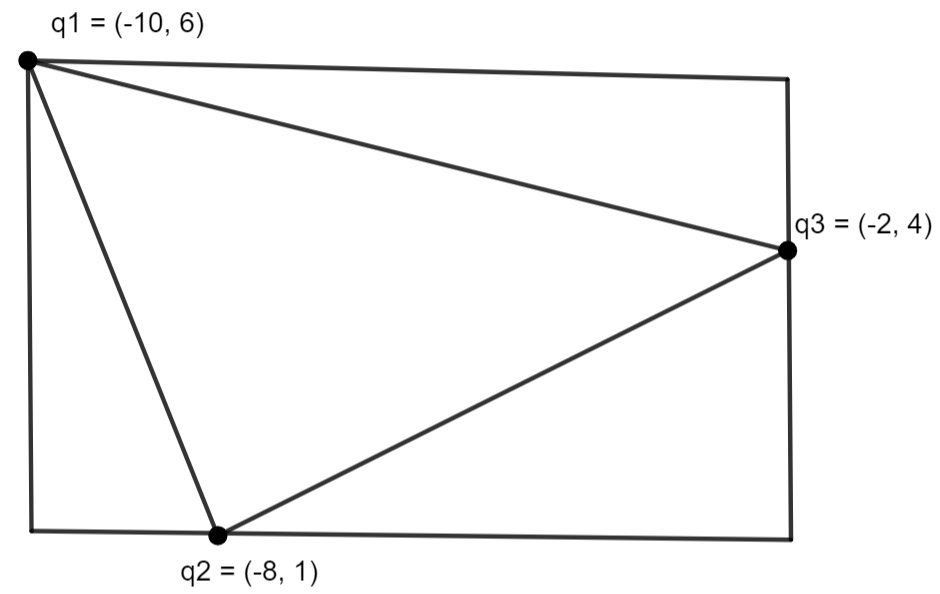
\includegraphics[width=0.5\linewidth]{Report/Part4/Capture.PNG}  
\caption{3 Points in Manhattan World}
\end{figure}

This means that by the triangle inequality, the distance between any two points is must be greater than the straight line distance. In fact, now we can take $\{|x_3 - x_1| + |y_3 - y_1|\} > \{|x_2 - x_1| + |y_2 - y_1|\} + \{|x_2 - x_3| + |y_2 - y_3|\}$ and compute where each section in brackets corresponds to on the rectangle. $|x_3 - x_1| + |y_3 - y_1|$ corresponds to the 2 legs formed from $q_1 \rightarrow q_3$. Then, $|x_2 - x_1| + |y_2 - y_1|$ corresponds to the legs formed from $q_1 \rightarrow q_2$ and $|x_2 - x_3| + |y_2 - y_3|$ is the legs of $q_2 \rightarrow q_3$. Now, we can further analyze the fact that the longest 2 legs possible, will form only half of the rectangle, meaning, our 3 points form a right triangle. With this in mind, we can look at our original inequality, $\{|x_3 - x_1| + |y_3 - y_1|\} > \{|x_2 - x_1| + |y_2 - y_1|\} + \{|x_2 - x_3| + |y_2 - y_3|\}$ and realize it muse be a contradiction! It is not possible for the length of 2 legs of a triangle to form more than half of the rectangle, and therefore, $\{|x_3 - x_1| + |y_3 - y_1|\} \leq \{|x_2 - x_1| + |y_2 - y_1|\} + \{|x_2 - x_3| + |y_2 - y_3|\}$. Therefore, Manhattan distances are consistent in grid worlds where the agent can move only in the four main compass directions.
\end{proof}


Our next concern will be with a variant of \emph{$A^*$ search} known as \emph{Adaptive $A^*$ search}. The idea behind this variant will be explained in more detail in the next section, but the main difference is that for an \emph{online search} problem, \emph{Adaptive $A^*$ search} will update the heuristic values of all the expanded nodes after each $A^*$ call. Remember, $A^*$ will only work with consistent heuristic values, therefore, this raises the question if our heuristic values are still consistent after updating them.

\begin{qoute}
\emph{Prove that Adaptive $A^*$ leaves initially consistent h-values consistent even if action costs can increase.}
\end{qoute}
\begin{proof}
After each \emph{$A^*$ search} we update our heuristics given by the function $h_{new}(s) = g(goal) - g(s)$. By doing so, we will always have an admissible heuristic since our $A^*$ path length is always optimal. Now, using the definition of a consistent heuristic, $h(s) \leq c(s,p) + h(p)$, we can substitute in $h_{new}(s)$ and $h_{new}(p)$ and obtain $g(goal) - g(s) \leq c(s,p) + g(goal) - g(p)$. By further simplification, $g(p) \leq c(s,p) + g(s)$. We then realize that this inequality looks very familiar, in fact, it is just our original $h(s) \leq c(s,p) + h(p)$ with the goal and start nodes reversed. We proved in the previous part that Manhattan distances were consistent in grid worlds with moving only in the 4 main compass directions, and the same proof applies for this inequality as well, with the difference being the start and goal nodes are switched.
\end{proof}


\section{Part 5: Heuristics in the Adaptive A*}
\label{sec: Part 5}

We now perform testing of \emph{Repeated Forward Adaptive $A_*$ search} and present the results compared to regular \emph{Repeated Forward $A^*$ search}. The difference with \emph{Adaptive $A^*$ search} is that after each call of the algorithm, we pass it new heuristic values which are updated based on the previous call to the function. By doing so, we are using previous knowledge and better guiding the algorithm in exploring new areas that are not known to lead to blockages.
\begin{figure}[H]
  \centering
  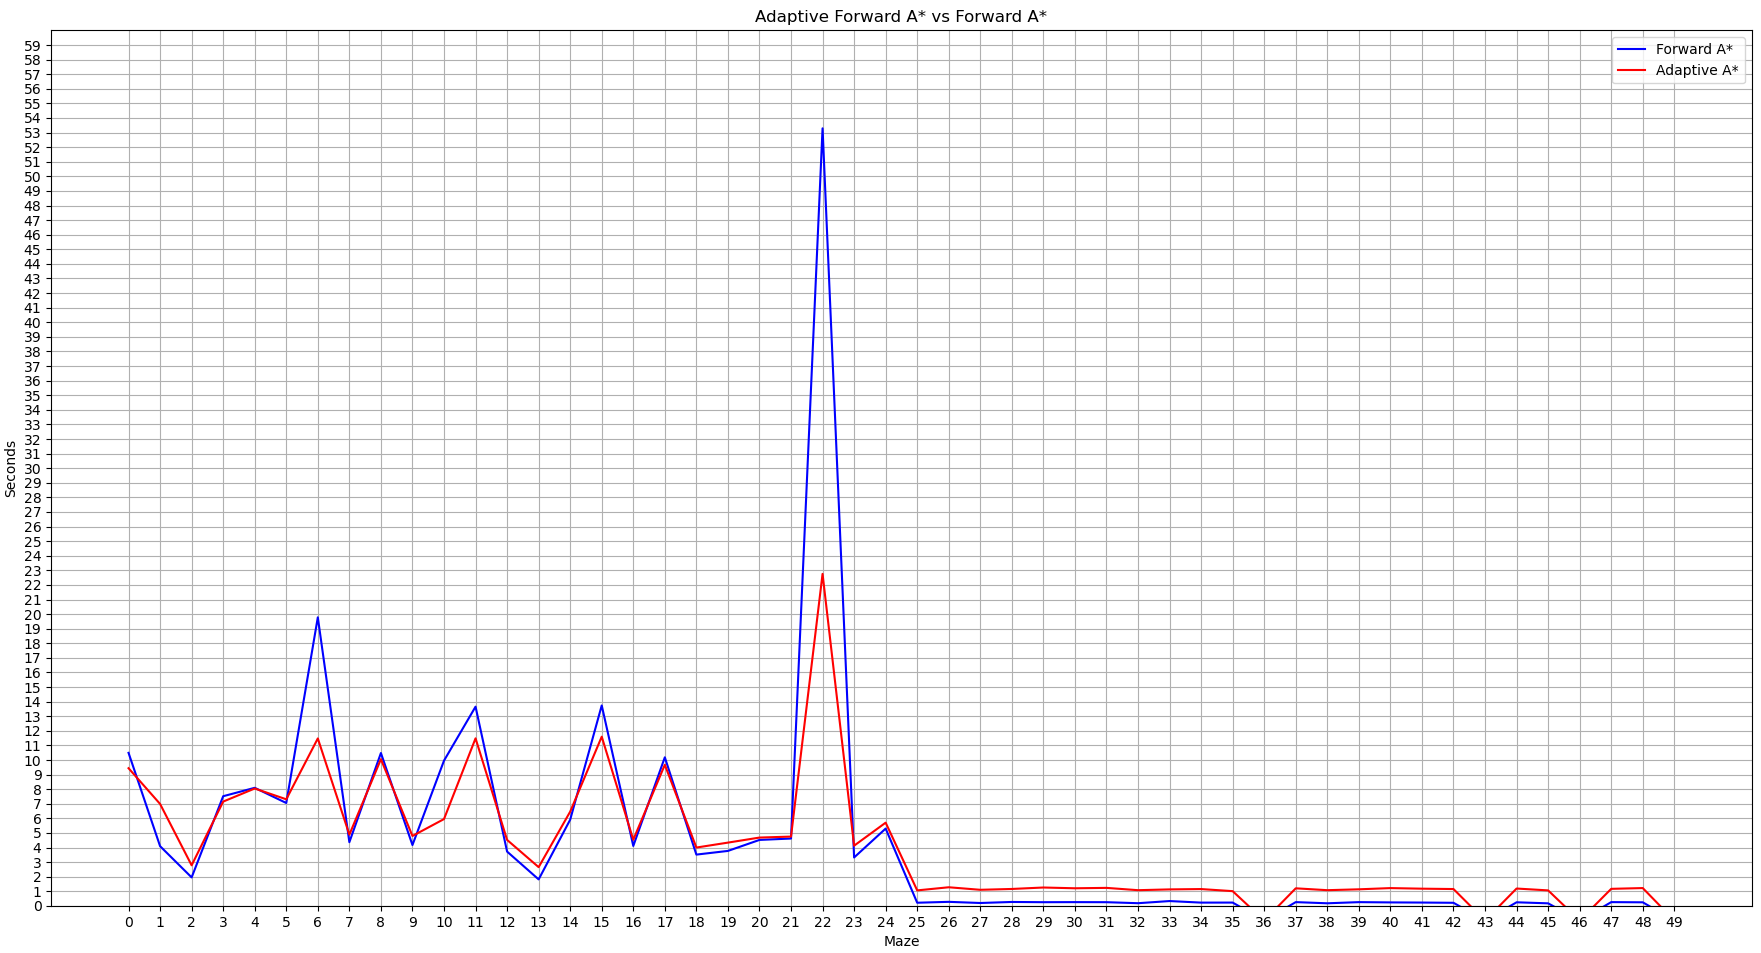
\includegraphics[width=1\linewidth]{Report/Part5/Figure_1.png}  
\caption{Repeated Adaptive Forward vs regular $A^*$ Comparison}
\end{figure}

Our results indicate that \emph{Adaptive $A^*$ search} does fair a bit better in complex mazes, such as our back tracked ones. However, we found that for simple random mazes, regular \emph{$A^*$ search} performs better. The reasoning for this is because in our random maze, each obstacle is usually simply overcome by going around the one or few walls, and a large alteration of the previous path is not needed. This means that by increasing the heuristics of previous expanded cells, we are forcing the algorithm to unnecessarily explore the surround areas first, rather than follow our classic depth first search method which regular $A^*$ performs. This is not a problem for our complex mazes because continuous walls exist. This means that most of the time, only one path exists and the agent is forced to move down a path. And updating the heuristics benefits the agent because at the few crossroads, where more than 1 path exists, the agent knows which path to take.
\section{Part 6: - Memory Issues}
\label{sec: Part 6}

In our finally portion of this project, we will analyze our memory usage and possible optimizations. The reason for this is that for many online path planning applications, such as real-time games, and even motion planning for robots with large configuration spaces, maps consist of a much larger state space than a 101 X 101 grid.


In this project we used Python for our implementation, and this on its own is not the most optimal solution for memory constrained environments. From a high level overview, Python is an interpreted language and has its syntax interpreted at run time. In the end, this means that the same code in Python will result in more assembly instructions than a similar implementation in the C language. Even so, we will dig into only memory usage in this section. 


We are fortunate to have used Python for this project since it allows use to quickly prototype and get a working demo. But we are unfortunate in the memory usage for even simple data types in Python. Since Python data type sizes vary from various Python distributions, to analyze our data type sizes in bytes, we use the \texttt{getsizeof} function from the \texttt{sys} module. Our results are below:

\begin{table}[H]
  \begin{center}
    \begin{tabular}{l|c|r}
      \textbf{Data Type} & \textbf{Bytes}\\
      \hline
      Bool & 12\\
      Tuple & 28\\
      Int & 14\\
      Node & 24\\
    \end{tabular}
    \caption{Python data type sizes}
  \end{center}
\end{table}

The odd thing about Python is that these sizes often vary with how much data is actually stored in each variable, and in fact, \texttt{numpy} arrays follow their own data type  optimizations for memory as well. 


If we were to use the above table, we would end up with some very inefficient designs. For example, a simple 1001 X 1001 grid would use approximately 12 MB of memory just for storing the grid. Therefore, we will use the standard C data type specifications for an Intel x86 machine running Linux provided in the table below: 
\begin{table}[H]
  \begin{center}
    \begin{tabular}{l|c|r}
      \textbf{Data Type} & \textbf{Bytes}\\
      \hline
      Char & 1\\
      Short & 2\\
      Int & 4\\
      Pointer & 4\\
      Node Struct & 14
    \end{tabular}
    \caption{C data type sizes}
  \end{center}
\end{table}

Our \texttt{Node} struct also takes into account padding, this means we use \texttt{short} variables, and a 2 byte padding is inserted between the last short and 4 byte pointer.


Now that we have defined our C data sizes, we can first discuss memory requirements for working with a 1001 X 1001 grid. If saving memory is our biggest concern, we can store the grid in a \texttt{char} array. Then, we can use bit wise operators to access each of the 8 bits in a char. Meaning, for each char, we can store the value of 8 cells (blocked or unblocked). This means, 
\begin{equation}
\lceil\frac{1001 * 1001}{8}\rceil = 125251 \; bytes \tag{1}
\end{equation}
Furthermore, it is very dependant on the map for how many structs in memory are allocated, but we will assume all cells end up allocated in the heap. We then obtain another 
\begin{equation}
1001 * 1001 * 14 = 14028014 \; bytes \tag{2}
\end{equation}
that are allocated in the binary heap, and since the binary heap exists as an array implementation, we will have to allocate a 1002001 length array of pointers:
\begin{equation}
1001 * 1001 * 4 = 4008004 \; bytes \tag{3}
\end{equation}
We also have to implement a method to track which nodes have been expanded, and for this we will need a Boolean matrix, which we can use from \emph{(1)}. Finally, we will need a matrix of heuristic values, and for this we will use a 1002001 length \texttt{short} array. This will put us at:
\begin{equation}
1001 * 1001 * 2 = 2004002 \; bytes \tag{4}
\end{equation}

Finally, from \emph{(1), (2), (3), and (4)}:
\begin{equation}
\frac{125251 * 2 + 14028014 + 4008004 + 2004002}{1000000} = 20.2905\; MB \tag{5}
\end{equation}

This is an approximation for the amount of memory needed to operate regular \emph{Forward $A^*$ search} on a 1001 X 1001 grid.


We can further analyze the largest grid we can operate on in the memory constraints of \emph{4 MB} by using the same equations above.

\begin{equation}
 \frac{2 * \frac{x^2}{8} + 14x^2 + 4x^2 + 2x^2}{1000000} = 4 \; MB \tag{6}
\end{equation}
\begin{equation}
 81x^2 = 16000000 \tag{7}
\end{equation}
\begin{equation}
 \lfloor x^2 \rfloor = 197530 \tag{8}
\end{equation}
\begin{equation}
 \lfloor x \rfloor = 444 \tag{9}
\end{equation}

From this, we can conclude that the largest maze we are able to operate on within the constraints of \emph{4 MB} of memory is approximately a 444 X 444 maze.


\begin{thebibliography}{1}
\bibitem{koenig}S. Koenig and M. Likhachev. Adaptive A* [Short Paper]. In Proceedings of the International Joint Conference on Autonomous Agents and Multiagent Systems (AAMAS), pages 1311-1312, 2005.

\end{thebibliography}
\end{document}
